\section{Validation du positionnement du module SEIS}

\begin{obj}
Valider les réglages dela commande des trois actionneurs linéairesassociés aux pieds,
 (figure \ref{ccinp_mp2019_fig_03}),afin de respecter les exigences liées à leur positionnement
\end{obj}
\ifprof
\else
On limitera l’étude à un des trois actionneurs. La chaîne structurelle de l’actionneur électrique utilisé dans le système est donnéée sur la figure \ref{fig_09}.

\begin{figure}[!h]
\centering
\includegraphics[width=\linewidth]{fig_09.png}
\caption{Chaîne structurelle de l’actionneur électrique linéaire \label{fig_09}}
\end{figure}

 Chaque actionneur électrique, appelé aussi vérin électrique, est asservi en position.


\textbf{Notations et spécifications :}
\begin{multicols}{2}
\begin{itemize}
\item masse à déplacer pour chaque vérin : $M =\SI{1}{kg}$;
\item pesanteur de la Terre : $g = \SI{9,81}{m.s^{-2}}$;
\item rapport de réduction du réducteur : $r = 0,01$;
\item rendement du réducteur : $\eta_r = 0,95$;
\item pas de la vis du système vis-écrou : $p = \SI{12}{mm}$;
\item rendement du système vis-écrou : $\eta_v = 0,96$;
\item coefficient de frottement visqueux du moteur : $f=\SI{0,002}{Nms/rad}$;
\item moment d’inertie équivalent total ramené sur l’arbre moteur : $J = \SI{0,00004}{kg.m^2}$;
\item résistance de l’induit de la MCC (Machine à Courant Continu) : $R =\SI{1}{\Omega}$;
\item inductance de l’induit de la MCC : $L = \SI{20}{\mu H}$;
\item constante de couple : $K_c = \SI{0,35}{NmA^{-1}}$;
\item constante de force contre électromotrice : $K_e = \SI{0,35}{Vs/rad}$;
\item tension d’alimentation de l’induit de la MCC : $u(t)$ en \si{V};
\item courant absorbé par l’induit de la MCC : $i(t)$ en \si{A};
\item vitesse de rotation en sortie de la MCC : $\omega(t)$ en \si{rad/s};
\item position angulaire en sortie de la MCC :  $\theta(t)$ en \si{rad};
\item force contre électromotrice de la MCC : $e(t)$ en \si{V};
\item couple moteur de la MCC : $C_m(t)$ en \si{Nm};
\item couple résistant total ramené sur l’arbre moteur : $C_r(t) = \dfrac{Mgpr}{2\pi \eta_v \eta_r} h(t)$\footnote{$h(t)$ désigne la fonction de Heaviside qui prend la valeur 0 pour t<0, 1 sinon.} en \si{Nm}.
\end{itemize}
\end{multicols}

\textbf{Équations du moteur à courant continu :}
\begin{multicols}{2}
\begin{itemize}
\item équation électrique : $u(t)=e(t)+Ri(t)+L\dfrac{\dd i(t)}{\dd t}$;
\item équations de couplage électro-mécanique : $e(t)=K_e \omega(t)$, $C_m(t)=K_C i(t)$.
\end{itemize}
\end{multicols}
\fi



\subsection{Détermination du couple résistant appliqué à l’arbre moteur (système vis-écrou)}
\ifprof
\else
 Une représentation du système vis-écrou et de la charge est donnée figure \ref{ccinp_mp2019_fig_10}.


\begin{minipage}[c]{.47\linewidth}
\begin{center}
%\includegraphics[width=\linewidth]{ccinp_mp2019_fig_09.png}
\captionof{figure}{Système vis - écrou \label{ccinp_mp2019_fig_09}}
\end{center}
\end{minipage} \hfill
\begin{minipage}[c]{.47\linewidth}
 Notation et hypothèses :
 \begin{itemize}
 \item $\vect{P}$ représente le poids dû à la masse du SEIS. Il s’applique sur l’écrou ;
\item la masse du système vis-écrou est négligeable devant les autres masses ;
\item $\vect{F}$ représente l’effort développé par le vérin électrique (résultante de l’effort de 
la vis sur l’écrou).
\end{itemize}
\end{minipage}
\fi

\question{Effecuter un bilan des forces exercées sur l’écrou en équilibre statique afin d’obtenir l’expression liant $F$, la norme du vecteur $\vect{F}$ et la masse du système à déplacer, M. Préciser clairement le principe/théorème utilisé.}
\ifprof
\begin{corrige}%
En effectuant un bilan des actions mécaniques en $O$ pour l’écrou, on obtient 
\begin{itemize}
\item 	Pesanteur sur l'écrou : $\vect{F}$
\item 	Effort développé par le vérin sur écrou : $\vect{P}$.
\end{itemize}

Par application du PFS : $||\vect{F}|| =||\vect{P}||$  soit $F=M.g$.

\end{corrige}
\else
\fi

\question{Donner l'expression littérale de $C_r(t)$ et mettre celle-ci sous la forme ci-dessous. Calculer la valeur numérique de $C_r(t)$ : $C_r(t)=\dfrac{Mgpr}{2\pi \eta_v \eta_r}$.}
\ifprof
\begin{corrige}%
Le couple en exercé par la vis, $c_v$, est lié à l’effort développé sur l’écrou par la relation suivante : $c_v (t)=F\dfrac{D}{2}\dfrac{1}{\eta_v}$ où $D$ représente le diamètre de l’écrou (application de la relation du rendement de la vis). 

D’autre part $D$ est lié au pas de la vis par la relation suivante : $D/2=\dfrac{p}{2\pi}$ 
d’où l’expression de $c_v(t)$ : $c_v (t)=F \dfrac{p}{\pi}\dfrac{1}{\eta_v}=M.g.\dfrac{p}{2\pi}\dfrac{1}{\eta_v}$.
On remonte jusqu’au couple en entrée du réducteur à partir de l’expression su rendement : $\eta_v= \dfrac{c_v \omega_{vis}}{c_R \omega_m}$ et à partir de la connaissance du rapport de réduction : $r=\omega_{vis}/\omega_m$.
 
On en déduit la relation finale : $C_r (t)=\dfrac{Mgpr}{2\pi\eta_v\eta_r}$.

A.N. $C_r (t)=\dfrac{M.g.p.r)}{2.\pi.\eta_v.\eta_r}=\dfrac{1 \times  9,81 \times  0,012\times  1/100}{2 \times  \pi 0,95\times 0,96}=\SI{0,20}{mN.m}$.

\end{corrige}
\else
\fi

\subsection*{Modélisation de la motorisation}
\ifprof
\else
La structure du schéma-bloc obtenue à partir du modèle de connaissance de la MCC est présentée sur la figure suivante.

\begin{figure}[!h]
\centering
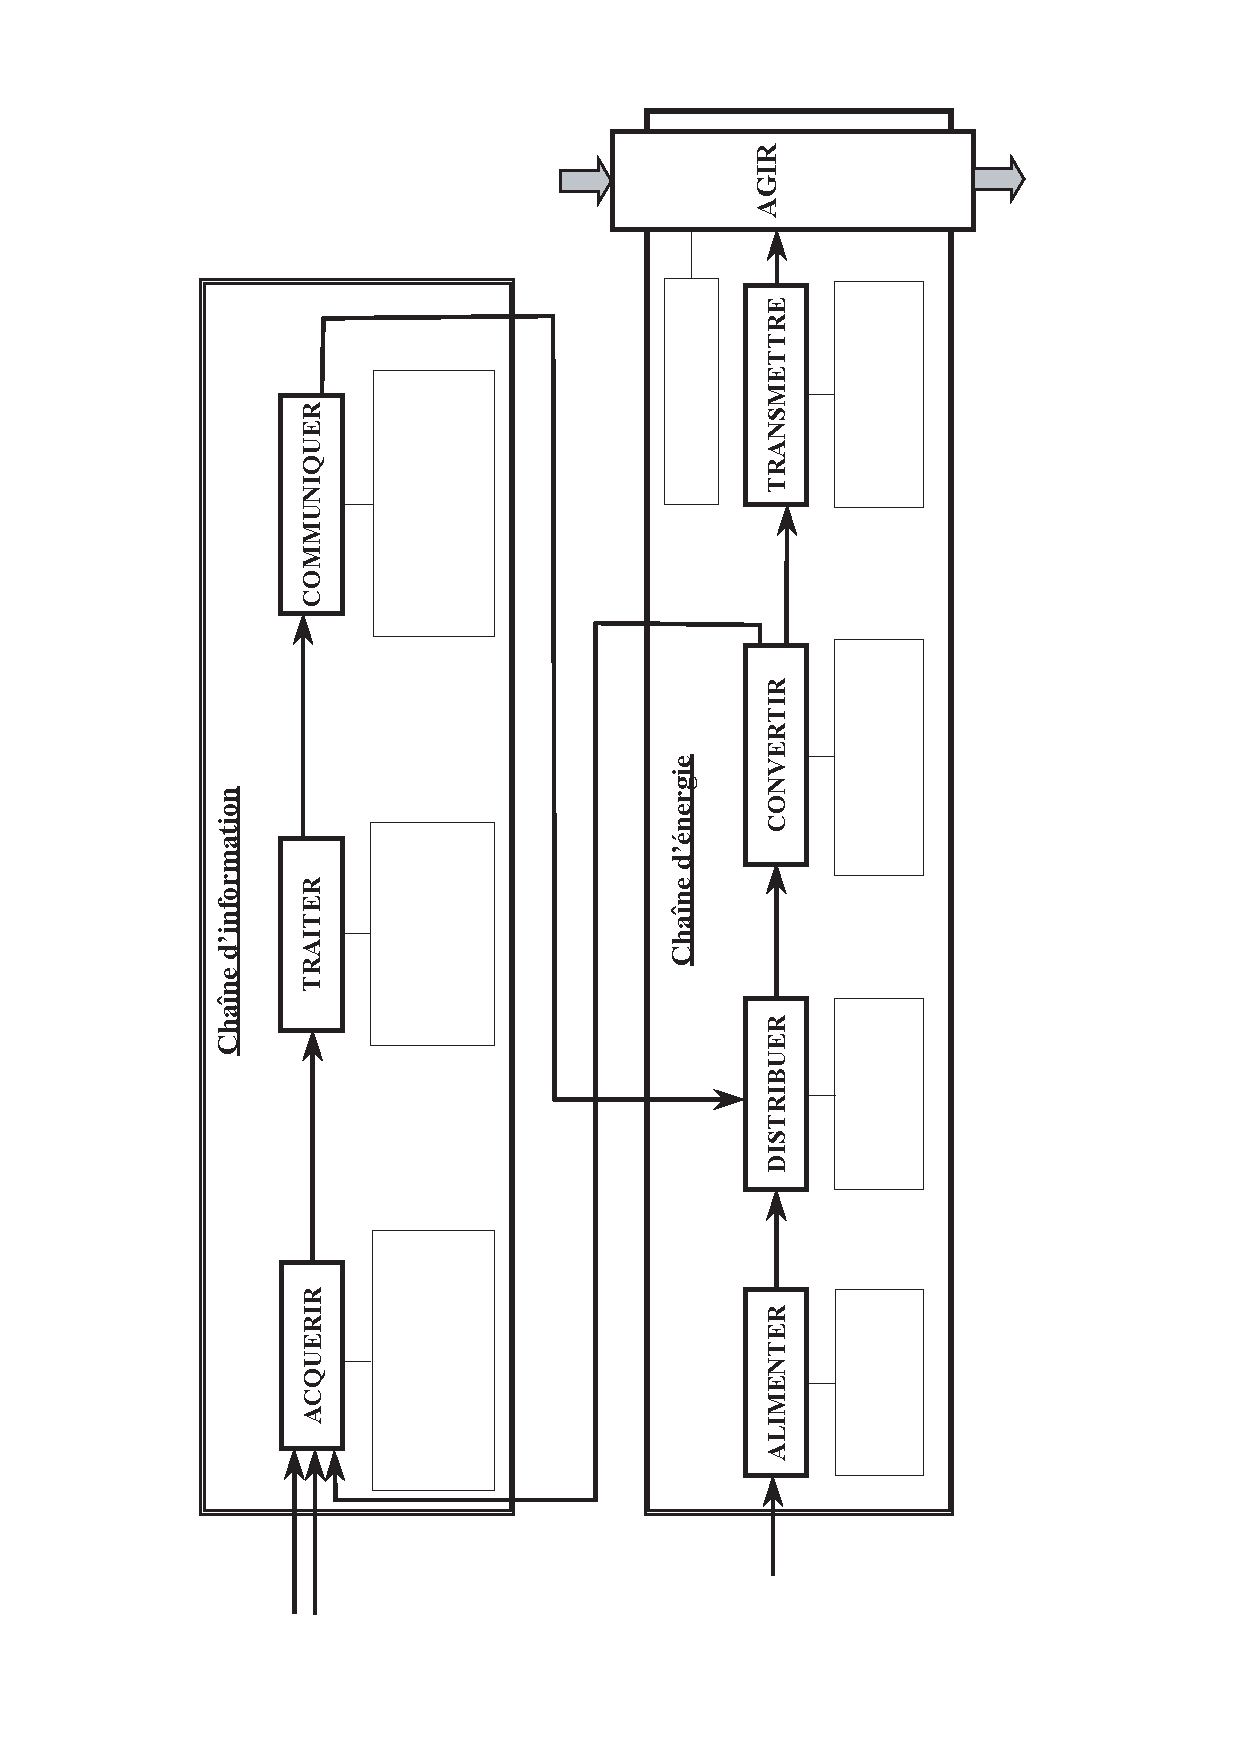
\includegraphics[width=.8\linewidth]{dr_01.png}
\caption{Structure du schéma bloc \label{dr_01}}
\end{figure}
\fi

\question{À partir des équations du moteur à courant continu, recopier et compléter (sous forme littérale) les blocs modélisant la MCC.}
\ifprof
\begin{corrige}%
On commence par l’écriture des équations (1) à (3) dans le domaine de Laplace :

(1) devient : $U(p)=E(p)+R I(p)+L.p I(p)$

(2) devient : $E(p)=K_e \Omega(p)$

(3) devient : $C_m (p)=K_c I(p)$

On identifie les variables d’entrée et de sortie de chaque bloc à compléter du document réponse et on cherche une équation liant ces deux variables à partir des trois équations précédentes :

(1) $U(p)-E(p)=RI(p)+L.pI(p)$ soit $I(p)=(U(p)-E(p))\times 1/(R+L.p)$

(2) $E(p)=K_e \Omega(p)$ 

(3) $C_m (p)=K_c I(p)$

On complète les trois blocs du document réponse.

\end{corrige}
\else
\fi

\ifprof
\else
L'application du théorème du moment dynamique à l'arbre moteur permet d'écrire l'équation suivante : 
$$
J\dfrac{\dd \omega(t)}{\dd t}  = C_m(t)-C_r(t)-f\omega(t).
$$
\fi

\question{Compléter le schéma-bloc.}
\ifprof
\begin{corrige}%
Plusieurs possibilités pour obtenir cette relation. Par exemple utilisation du principe fondamental de la dynamique :
$J\dfrac{\d\omega(t)}{\dd t}=C_m (t)-C_r (t)-f\omega(t)$ 
Soit dans le domaine de Laplace : $Jp\Omega(p)=C_m (p)-C_r (p)-f\Omega(p)$
D’où l’obtention de la fonction de transfert du bloc à compléter :  $\dfrac{\Omega(p)}{C_m (p)-C_r (p) }=\dfrac{1}{Jp+f}$.

\end{corrige}
\else
\fi

\ifprof
\else
On se place dans le cas particulier où $C_r(p) = 0$.
\fi

\question{Donner l’expression, sous sa forme canonique, de la fonction de transfert en boucle fermée $\indice{F}{m1}(p)=\dfrac{\Omega(p)}{U(p)}$.}
\ifprof
\begin{corrige}%
L’expression de $F_{m1}(p)$ est obtenue à l’aide de la formule de Black :
$F_{m1} (p)=\dfrac{\dfrac{K_C}{(R+Lp)(f+Jp)}}{1+\dfrac{K_CK_E}{(R+Lp)(f+Jp)}}=\dfrac{K_C}{(R+Lp)(f+Jp)+K_C.K_E }=\dfrac{\dfrac{K_C}{Rf+K_C.K_E}}{1+\dfrac{RJ+Lf}{Rf+K_CK_E }p+\dfrac{LJ}{Rf+K_CK_E} p^2 }$

\end{corrige}
\else
\fi

\ifprof
\else

La figure \ref{dr_02} présente les résultats expérimentaux de l’évolution de la vitesse de rotation, $\omega(t)$ à la suite de l’application d’un échelon de tension $u(t)$ d’une amplitude de \SI{12}{V} aux bornes de la MCC. On pose $\indice{F}{m2}(p)=\dfrac{\Omega(p)}{U(p)} = \dfrac{F_0}{1+T_0p}$

\begin{figure}[!h]
\centering
\includegraphics[width=.8\linewidth]{dr_02.png}
\caption{Réponse de la MCC à un échelon de \SI{12}{V}\label{dr_02}}
\end{figure}
\fi

% Q18
\question{Justifier le choix d’une fonction de transfert d’ordre 1 pour modéliser le comportement de la MCC à partir des essais expérimentaux. Effectuer les constructions graphiques nécessaires sur 
la figure \ref{dr_02} afin de déterminer la valeur du gain statique $F_0$
et de la constante de temps $T_0$ de $\indice{F}{m2}(p)$. Proposer une hypothèse simplificatrice permettant de justifier le passage à l’ordre 1 de $\indice{F}{m2}(p)$ par rapport à $\indice{F}{m1}(p)$.}
\ifprof
\begin{corrige}%
On en déduit l’expression de $F_{m2}(p)$ :
$F_{m2}(p)=\dfrac{2,75}{1+0,00023.p}$.
Pour obtenir $F_{m2}(p)$ à partir de $F_{m1}(p)$, il est nécessaire de réduire l’ordre de la fonction de transfert ce qui implique de négliger un pôle de $F_{m1}(p)$ (notion de pôle dominant).

\end{corrige}
\else
\fi

\subsection{Étude de l’asservissement en position du vérin}

\begin{obj}
Choisir un correcteur approprié permettant de satisfaire le cahier des charges vis-à-vis des exigences concernant l’asservissement en position du vérin électrique suivant l’axe $\vect{y_0}$ conformément à la figure 11.
\end{obj}

\ifprof
\else

\begin{figure}[!h]
\centering
\includegraphics[width=.8\linewidth]{fig_11.png}
\caption{Déplacement de la tige du vérin\label{fig_11}}
\end{figure}

La mesure de la distance est obtenue grâce à un capteur à ultrason permettant de délivrer, sous la 
forme d’impulsions, une image de la distance entre la structure sur SEIS et le sol. Cette information 
est ensuite traitée afin de générer un signal image de la distance parcourue par la tige du vérin.

L’étude précédente a permis d’obtenir un modèle de comportement de la MCC intégré dans le schéma bloc de l’asservissement présenté en figure \ref{fig_12} pour lequel $C_r(p)=0$.

\begin{figure}[!h]
\centering
\includegraphics[width=\linewidth]{fig_12.png}
\caption{Schéma-bloc de l’asservissement en position du vérin électrique\label{fig_12}}
\end{figure}


\textbf{Notations et spécifications :}
\begin{multicols}{2}
\begin{itemize}
\item gain du capteur: $\indice{K}{capt} = \SI{588}{impulsions/m}$;
\item gain de l’ensemble réducteur et vis-écrou : $\indice{K}{red} = \SI{19.1e-6}{m/rad}$;
\item vitesse linéaire de la tige du vérin : $V(t)$ en \si{m.s^{-1}};
\item déplacement linéaire de la tige du vérin : $d(t)$ en $\si{V}$;
\item correcteur: $C_0(p)$;
\item gain du hacheur: $\indice{K}{H} = 1,163$.
\end{itemize}
\end{multicols}

Pour toute la suite du sujet, on considère : $\indice{C}{r}(p)=0$. Tout d'abord, le correcteur est consdéré unitaire $\indice{C}{0}(p)=1$.
\fi

%\question{Donner l'expression littérale de la fonction de transfert en b}
%\ifprof
%\begin{corrige}%
%
%\end{corrige}
%\else
%\fi
\question{}

\question{Donner l’expression littérale de $M(p)$ et, pour garantir un bon asservissement, l’expression 
littéralede $\indice{K}{adapt}$.}
\ifprof
\begin{corrige}%
On choisit $\indice{K}{adapt}=\indice{K}{capt}$ afin d’interpréter la vitesse de rotation du moteur comme une tension avec le même gain que celui de la chaîne de retour.

Dans le domaine temporel la vitesse linéaire et le déplacement sont lié par l’équation suivante :
$v(t)=\dfrac{\dd(t)}{\dd t}$ soit dans le domaine de Laplace : $V(p)=pD(p)$.
On en déduit la fonction de transfert de $M(p)$ : $M(p)=\dfrac{D(p)}{V(p)} =\dfrac{1}{p}$.

\end{corrige}
\else
\fi

\question{ Déterminer l’expression littérale de la fonction de transfert en boucle ouverte $\indice{G}{BO}(p)$ et mettre celle-ci sous forme canonique. Donner la classe de cette fonction de transfert. En déduire\footnote{La déduction sera (re)vue en seconde année. Il vous faudra donc sûrement la calculer.}
 la précision du système.}
\ifprof
\begin{corrige}%
L’expression de la FTBO de ce système asservi est donnée par :
%
%$\indice{G}{BO}(p)=M(p)\indice{K}{red}\indice{K}{capt}C_0 (p)K_p×\dfrac{\dfrac{K_C.K_E}{R.f+K_C.K_E}}{\dfrac{J.R}{R.f+K_C.K_E}.p+1}$
%
%$=\dfrac{\dfrac{K_C.K_EK_p.\indice{K}{capt}.\indice{K}{red}}{p(Rf+K_CK_E}}{p.(\dfrac{JR}{R.f+K_C.K_E}.p+1) }$.
%Ou 
$\indice{G}{BO}(p)= \dfrac{F_0 K_H\indice{K}{capt}\indice{K}{red}}{p.(T_0.p+1)}$
Cette fonction de transfert d’ordre 2 présente un terme p en facteur au dénominateur, donc de classe 1.
Pour un système asservi, si la classe de la FTBO est 1, le système présente une erreur statique, ou de position, nulle. Le système est donc précis et répond à une exigence du cahier des charges fonctionnel

\end{corrige}
\else
\fi
 
  On donne l’expression numérique dela fonction de transfert en boucle ouverte :
  $\indice{G}{BO}(p)=\dfrac{0,0112}{p\left( 0,00028 p +1\right)}$.

\question{Tracer les diagrammes de Bode asymptotiques et réels de la fonction de transfert $\indice{G}{BO}(p)$ sur le DR3. En déduire la marge de phase de l’asservissement en effectuant toutes les constructions 
graphiques nécessaires. Conclure sur le respect de l’exigence 006 «Stabilité ».}
\ifprof
\begin{corrige}%
\begin{center}
\includegraphics[width=.8\linewidth]{cor_q21.png}
\end{center}
\end{corrige}
\else
\fi

\ifprof
\else

\begin{figure}[!h]
\centering
\includegraphics[width=.8\linewidth]{dr_03.png}
\caption{Diagramme de Bode \label{dr_03}}
\end{figure}

 On désire quantifier la rapidité du système à la suite d’une sollicitation en échelon. On donne les 
relations permettant de calculer le temps de réponse à 5\%, noté $\indice{t}{r5\%}$, pour un système d’ordre deux (avec $\xi$ le facteur d’amortissement et $\omega_0$ la pulsation propredu système non amorti):

$$
\left\{ 
\begin{array}{l}
\xi < \dfrac{1}{\sqrt{2}}, \indice{t}{r5\%} \simeq \dfrac{3\xi}{ \omega_0} \\
\xi > \dfrac{1}{\sqrt{2}}, \indice{t}{r5\%} \simeq \dfrac{6\xi }{\omega_0} \\
\end{array}
\right.
$$ 
\fi


\question{ Déterminer et calculer les paramètres caractéristiques de la fonction de transfert en boucle 
fermée $\indice{G}{BF}=\dfrac{D(p)}{D_c(p)}$. En déduire le temps de réponse de l’asservissement en vitesse. Conclure sur le respect de l’exigence 004 «~Rapidité~».}
\ifprof
\begin{corrige}%
Détermination de $\indice{G}{BF} (p)$ à partir de $\indice{G}{BO} (p)=\dfrac{0,0112}{(p(0,00028p+1)} $.

$\indice{G}{BF} (p) = \dfrac{\indice{G}{BO} (p)}{1+\indice{G}{BO} (p)} = \dfrac{1}{1+89 p + 0,025 p^2}$


On en déduit les expressions de la pulsation propre et du facteur d’amortissement par identification :
$
\left\{
\begin{array}{l}
\dfrac{1}{\omega_0^2} = 0,025 \\
\xi = \dfrac{1}{2}\omega_0 89
\end{array}
\right.$

 soit $\omega_0 = \SI{6,3}{rad/s}$ et $\xi =281$.
 
D’après les relations donnant l’expression du temps de réponse, (4), pour $\xi >\dfrac{1}{\sqrt{2}}$ : $t_{r5\%}\simeq(6 \xi)/\omega_0 \simeq \SI{268}{s}$
Le système est donc beaucoup trop lent au regard de l’exigence en rapidité (« Id 004 ») : 
$t_{r5\%}<\SI{5}{s}$.

\end{corrige}
\else
\fi
\ifprof
\else
Afin d’améliorer les performances de l’asservissement, on choisit un correcteur proportionnel de gain 
$\indice{K}{D}$ tel que $C_0(p) = \indice{K}{D}$. La valeur numérique du gain sera déterminéeà partir de deux méthodes :
\begin{itemize}
\item approche graphique, à partir de la marge de phase (maîtrise de la stabilité);
\item approche analytique, à partir d’un comportement imposé.
\end{itemize}
\fi

\question{À partir de constructions graphiques sur la figure \ref{dr_03}, donner la valeur du gain du correcteur $\indice{K}{D1}$, permettant de garantir une marge de phase supérieure à 70\degres. La valeur de $\indice{K}{D1}$ vous paraît-elle pertinente et réaliste ?}
\ifprof
\begin{corrige}%
On relève sur la phase du diagramme de bode la pulsation $\omega_1$ correspondant à une marge de phase de 70\degres (la phase de la ftbo est alors de -120°) : $\omega_1\simeq \SI{0.02}{rd/s}$. Pour cette même pulsation on relève le gain sur l’évolution du gain du diagramme de bode $G_1 \simeq -\SI{107}{dB}$.

On en déduit le gain $K_{D1}$ permettant de garantir une marge de phase supérieure à 70\degres :
$20\log_10 (K_{D1})\simeq \SI{107}{dB}$ soit $K_{D1}\simeq 10^(107/20)\simeq 223000$ !!
Cette valeur permet d’obtenir un système avec peu de dépassement et beaucoup plus rapide en théorie. Bien évidemment cette valeur n’est pas du tout réaliste puisqu’il faut tenir compte des saturations présentes sur le système réel (le hacheur en particulier) limitant la valeur du gain proportionnel que l’on peut mettre en œuvre dans le domaine linéaire.

\end{corrige}
\else
\fi

\ifprof
\else
 On impose un temps de réponse à 5\% de \SI{5}{s} et un facteur d’amortissement $\xi$ supérieur à 1.
 On donne l’expression numérique de $\indice{G}{BF}(p)$ avec un correcteur de gain $\indice{K}{D}$ :
 $\indice{G}{BF}(p)=\dfrac{1}{\dfrac{0,025}{K_D}p^2+\dfrac{89}{K_D}p +1}$.
 \fi
 
\question{À partir des équations liant le temps de réponse, le facteur d’amortissement et la pulsation 
propre ainsi que de l’expression numérique de $\indice{G}{BF}(p)$, donner une expression liant $t_{r5\%}$  et $\indice{K}{D2}$. En déduire la valeur de $\indice{K}{D2}$ permettant de respecter la contrainte imposée en termes de rapidité.}
\ifprof
\begin{corrige}%
On se place dans le cas particulier où $\xi>\dfrac{1}{\sqrt{2}}$ avec $t_{r5\%}\simeq \dfrac{6 \xi}{\omega_0}$ . On extrait les valeurs de $\xi$ et $\omega_0$ à partir de l’expression de $G_{BF}(p)$ (5) :
$\left\{
\begin{array}{l}
\dfrac{1}{\omega_0 }^2=\dfrac{0,025}{K_D} \\
\xi =\dfrac{1}{2}\omega_0 \dfrac{89}{K_D}   \\
\end{array}
\right.
$

soit $\dfrac{\xi}{\omega_0} =\dfrac{89}{K_D}$  d’où $t_{r5\%}\simeq \dfrac{6\xi}{\omega_0} \simeq 3 \dfrac{89}{K_D}\simeq 267/K_D$.
  
Si on impose un temps de réponse à 5\% de \SI{5}{s} il faut choisir comme gain : $K_{D2}\simeq 267/t_{r5\%} \simeq 53,4$.
Cette valeur semble plus raisonnable….

\end{corrige}
\else
\fi

\ifprof
\else
 On donne ci-dessous les tracés de la sortie du système asservi à la suite d’un échelon de consigne de 
\SI{10}{cm} pour $\indice{K}{D1} = \num{220000}$ et $\indice{K}{D2} = 53$.


\begin{figure}[!h]
\centering
\includegraphics[width=\linewidth]{fig_13.png}
\caption{Réponses indicielles du système asservi \label{fig_13}}
\end{figure}
\fi

\question{Commenter les courbes (respect des exigences) et choisir le correcteur qui vous paraît le plus 
pertinent.}
\ifprof
\begin{corrige}%
Pour les deux correcteurs l’erreur statique est nulle, le système est donc précis.
On observe un dépassement d’environ 10\% pour le premier correcteur et aucun pour le deuxième qui convient mieux vis-à-vis de ce critère (stabilité).
En terme de rapidité le premier correcteur est bien plus performant (tr5\%=\SI{0,0018}{s} pour le premier et tr5\%=\SI{5}{s} pour le second) mais le second correcteur, bien que moins rapide, respecte le cahier des charges…
Le correcteur le plus approprié est bien évidemment le second car il répond en tout point au cahier des charges et présente un gain de valeur numérique raisonnable.

\end{corrige}
\else
\fi
